\chapter{Background}

\section{vroom}
vroom currently uses hugepages and locks them using mlock to prevent the Kernel from swapping them out.
This only enables the use of 2MiB hugepages, which can be disadvantageous for certain applications that would benefit from smaller page sizes.
A NVMe driver consists of submission and completion queues, implemented as ring buffers.
The driver adds commands to the submission queue, which the NVMe controller reads and executes.
The executed command gets placed on a corresponding completion queue.
For accessing the devices memory as well as the device accessing the host memory, it is necessary to either use the physical addresses and compromise on safety and use root privileges or use the IOMMU for virtualization, which can introduce performance overhead.
We unbind the kernel driver and bind it to pci-stub. Pci-stub does not do anything but occupy the pci-driver such that the kernel or another application can not bind to the device.

\section{Persistent and Transparent Hugepages}

\section{Peripheral Component Interconnect Express}

\section{Direct Memory Access}
Using Direct Memory Access we can bypass the CPU for I/O operations. Previously this was handled by a separate DMA-controller hardware (third-party DMA) but using PCI, we can directly access it through bus mastering (first-party DMA).

\section{I/O Memory Management Unit}
Memory Management Units (MMU) for the CPU have been in use since the 1980s. After their first integrated application featuring on Intels 80286 chip \cite{intel80286}, they since have become the defacto standard for addressing memory on computers. By providing processes with a virtual address space instead of physical addresses, every process is isolated and can not access without having the privilege to. The MMU uses pages for the translation of addresses. Each address points to a region of memory called a page. These pages can have different sizes, with the default being 4Kib pages.
The translation of these pages are stored in a page table structure. A page table structure consists of multiple tables that store parts of the physical address. Certain parts of an address are used as offset in these tables. When an address is translated, a page table walk has to performed. On a 4 level page table structure as the IOMMU uses for 4KiB pages, one address resolution uses 4 memory accesses. Thus, a page table walk is a performance costly operation. To circumvent this, there exists an Translation Lookaside Buffer (TLB). This TLB can store a certain amount of page translations, and is very performant to access. Frequent access to the same address can be done at a fraction of the time needed to perform a page table walk. If an address is not stored in the TLB, it is called a TLB miss, and the IOMMU has to perform a page table walk.
The advantages and success of the CPUs MMU as well as the introduction of the PCIe bus specification have incentivised Hardware manufacturers to apply this concept on peripheral device busses. In 2006, Intel introduced their "Virtualization Technology for Directed I/O" (VT-d) and AMD their "AMD I/O Virtualization Technology" (AMD-Vi/IOMMU). In this thesis, the term IOMMU references both technologies.
Using DMA Remapping (DMAR) the CPU is bypassed and the direct memory access translated by the IOMMU.

% The IOMMU does this by performing page table walks, through which a physical address is translated to a virtual address. To manage the huge address spaces required by modern computing, multi-level page tables are used. This results in a huge virtual address space size, but a single address resolution using multiple memory accesses. In the case of Intels VT-d the page table structures consists of 4, 3 and 2 tables for 4kib, 2mib and 1gib pages respectively as seen on \autoref{fig:pagewalk4kib}.
% In order to not perform such an expensive operation on every address resolution, a buffer is used to cache previous translations. This buffer is called the I/O Translation Lookaside Buffer (IOTLB). Using the buffer results in a fraction of the time needed to perform a page walk. 

\begin{figure}
    \centering
    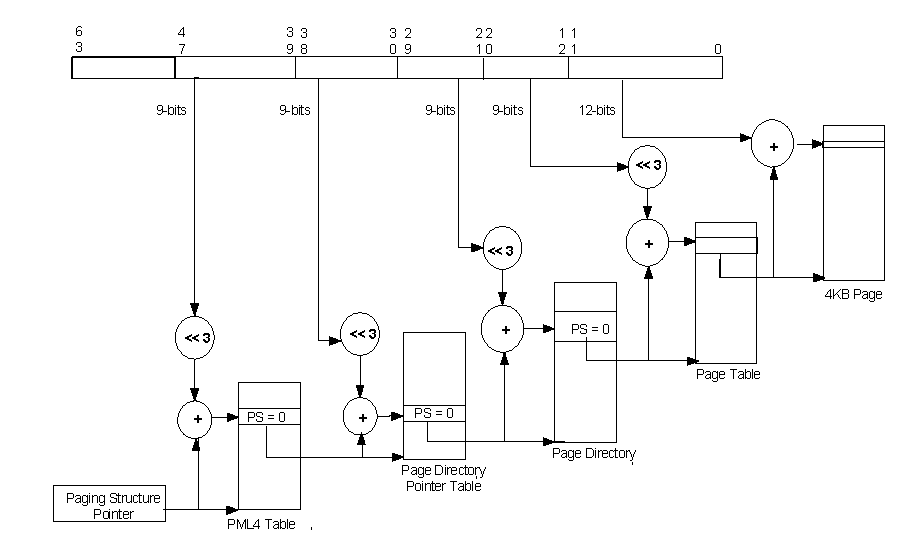
\includegraphics[width=\textwidth]{figures/4kibtranslation.pdf}
    \caption{VT-d Paging structure for translating a 48-bit address to a 4-KByte page}
    \label{fig:pagewalk4kib}
\end{figure}

\section{I/O Translation Lookaside Buffer}
As page table walks are rather costly in performance, a cache on the IOMMU is used to store previously calculated addresses. This cache is called the Input/Output Translation Lookaside Buffer. The IOTLB possesses a limited capacity for entries which is not officially documented.

\subsection{Character and Block Devices}
Unix/Linux use two types of devices: Character and Block devices. Character devices are used for devices with small amounts of data and no frequent seek queries, like keyboard and mouse. Block devices on the other hand have a large data volumes, which are organized in blocks and where search is common, like hardddrives and ram disks.
Read and Write operations on character devices are done sequentially byte-by-byte, while on block devices, read/write is done at the data block level.
These constraints also impact how the drivers for these devices work. CDev drivers directly communicate with the device drivers, while block device drivers work in conjunction with the kernel file management and block device subsystem. This allows efficient asynchronous read/write operations for large data amounts, but small byte sized data transfer achieves lower latency on character devices.

\subsection{Rust}
Rust as a programming language offers a lot of benefits, especially in the systems programming field. The memory safety enforced by the borrow checker and the focus on providing the most concise and exact syntax like default variable immutability while obmitting boilerplate make it an excellent choice for modern systems development.